%\documentclass[tikz, border=5pt]{standalone}
\begin{document}
	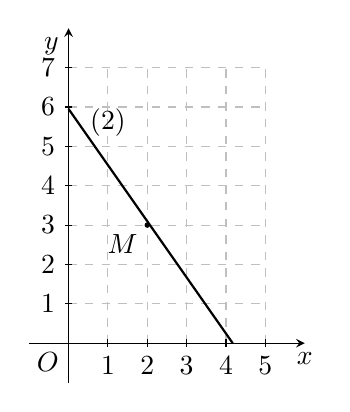
\begin{tikzpicture}[>=stealth, scale=0.5]
		% 1. 绘制坐标轴
		\draw[->] (-1,0) -- (6,0) node[below ] {$x$};  % x轴(带箭头和标签)
		\draw[->] (0,-1) -- (0,8) node[below left] {$y$};  % y轴(带箭头和标签)
		\node at (0,0) [below left] {$O$};           % 原点标记
		
		% 2. 绘制网格线(虚线)
		\foreach \x in {1,2,...,5} {
			\draw[dashed, gray!50] (\x,0) -- (\x,7);  % 垂直网格线
			\draw (\x, 0.1) -- (\x, -0.1) node[below] {$\x$};  % 小竖线(长 0.2 单位)x轴刻度标记
		}
		\foreach \y in {1,2,...,7} {
			\draw[dashed, gray!50] (0,\y) -- (5,\y);  % 水平网格线
			\draw (0.1,\y) -- (-0.1,\y) node[left] {$\y$};  % 小竖线(长 0.2 单位)y轴刻度标记
		}
		
		% 3. 绘制直线(从 (0,6) 到 (4,0))
		\draw[thick] (0,5.95) -- (4.17,0);
		
		% 4. 标记点 M(2,3)
		\fill (2,3) circle (2pt);           % 绘制点 M
		\node at (2,3) [below left] {$M$}; % 标注点 M
		
		% 5. 标注区域 (2)
		\node at (1,5) [ above] {(2)};
		
	\end{tikzpicture}
\end{document}
